\chapter{Phase 2 Development}
\label{chap:work}

This chapter details the development work that has been performed in the second phrase of the project.  This includes conceptual problems faced and their solutions.

%For each of the below, why, how inc conceptual problems, impact, how it could be improved

\section{Design Decisions}

During this phase of development a number of design decisions had to be made.  The decisions broadly fell into two categories:  \ac{UI} decisions and architectural decisions.  Ideally there should be a method behind such decisions.  The decisions and the reasoning behind them are below:

\subsection{\ac{UI} Design}

During the planning phase of the project (MPP) wireframe versions of the components of the \ac{UI} were developed.  The purpose of these wireframes was to allow for the \ac{UI} to be be evaluated somewhat before development started.  It is cheaper to fix problems early, fixing the problem before any development is particularly cheap.

During the second phase of development (MPP2) the \ac{UI} was refined and new elements were added to it.  It would have been desirable to again first create wireframes and evaluate them with the users before starting development.  This approach was not feasible in this stage of development.  It would have been necessary to hold more frequent user evaluations placing a greater strain on the user's time.

Instead the \ac{UI} was developed and then users evaluated it.  The \ac{UI} was then changed as required.  This iterative approach allowed for the \ac{UI} to be developed with being bottlenecked by waiting for wireframes to be  evaluated.  The improvement of the architecture outlined in Section~\ref{sec:architecture} made changes easier.  The \ac{UI} was contained much less information about the state of the tool.  The \ac{UI} effectively call an \ac{API}.  A \ac{UI} change no longer led to a reworking of logic.

\subsection{Architectural Design}
\label{sec:architecture}
After the first stage of development there was little architectural design.  The three main elements of the tool were the \ac{UI}, the graph visualisation and the model visualisation.   As you can see in Figure~\ref{fig:initial_architecture} each component was passing information to the other components.  Some of the items being passed around had references to to other components.  At the start of this phase of development (MPP2) the features that were to be implemented were too complex for this `lack of architecture' architecture.

The program was refactored to focus on an architectural model where there all the data is centralised in a single location.  This can be seen in Figure~\ref{fig:final_architecture}.  With these components if the original architecture was continued the interaction would look like Figure~\ref{fig:initial_architecture_future}.  The visualisation and \ac{UI} components select what they need to display from this central location.  This greatly reduced the amount of information that was having to be passed between all the components.  A refresh of the \ac{UI} components is then all that is needed to display the most update information.  This is similar to the \ac{MVC} architecture.  A simple diagram for \ac{MVC} can be seen in Figure~\ref{fig:mvc}.  With \ac{MVC} In this case the controller and the view are not entirely separated.

Figure~\ref{fig:detailed_architecture} shows a more detailed architectural diagram of the system.  The model is the session state.  This contains all the information for the visualisations such as the lines and results, the annotations and miscellaneous \ac{UI} toggles.  The controller is the \ac{UI} actions here affect the model.  The controller also triggers refreshed in the view.  The view here are the visualisations.  They display the information from the model.

\tdi{talk about singleton}

\begin{figure}[h!]
    \centering
    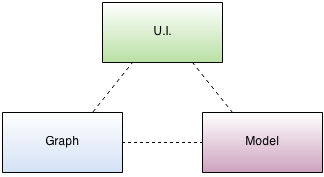
\includegraphics[width=0.4\textwidth]{images/initial_architecture.png}
    \caption{Architecture layout at the start of MPP2}
    \label{fig:initial_architecture}
\end{figure}

\begin{figure}[h!]
    \centering
    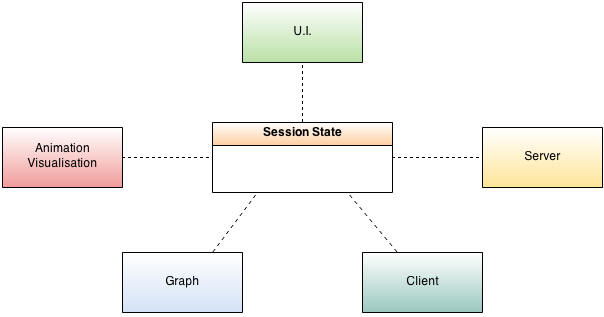
\includegraphics[width=0.6\textwidth]{images/final_architecture.png}
    \caption{Architecture layout at the end of MPP2}
    \label{fig:final_architecture}
\end{figure}

\begin{figure}[h!]
    \centering
    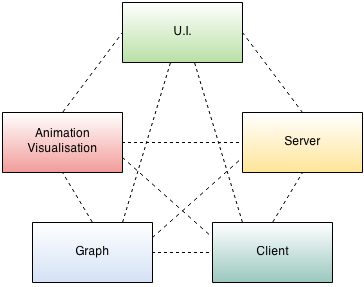
\includegraphics[width=0.4\textwidth]{images/initial_architecture_future.png}
    \caption{Architecture layout at the end of MPP2 if initial architecture was continued.}
    \label{fig:initial_architecture_future}
\end{figure}

\begin{figure}[h!]
    \centering
    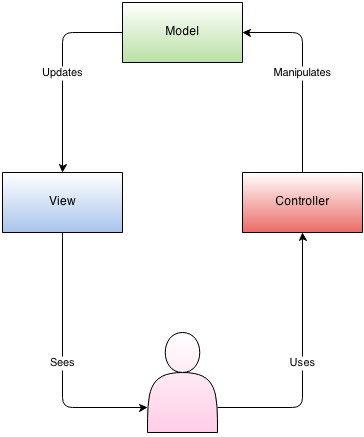
\includegraphics[width=0.4\textwidth]{images/mvc.png}
    \caption{Basic \ac{MVC} architecture}
    \label{fig:mvc}
\end{figure}

\afterpage{%
    \clearpage% Flush earlier floats (otherwise order might not be correct)
    \begin{landscape}
        \begin{figure}
            \centering
            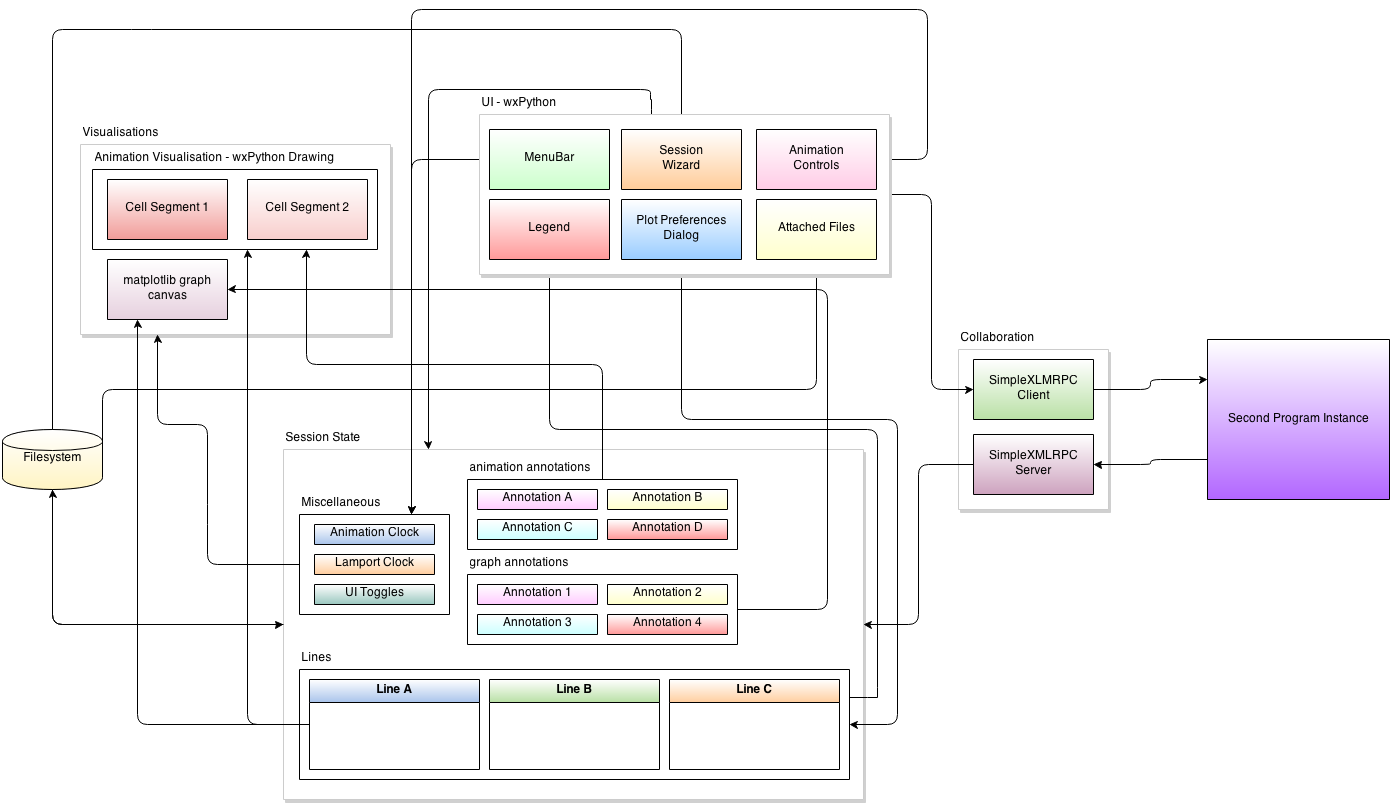
\includegraphics[height=0.9\textheight]{images/detailed_architecture.png}
            \caption{Detailed breakdown of program components and how they interact}
            \label{fig:detailed_architecture}
        \end{figure}
    \end{landscape}
}

\section{Finished Product}
\tdi{Not sure how necessary this is.  The plan would be a screenshot by screenshot walkthrough - may fit better in the self evaluation.  it will possibly just be duplicating screenshots that exist elsewhere}

\section{Animation}
\label{sec:animation}

Animation was a key goal of the project.  The core aim of the project is to help biologists who aren't comfortable with traditional time-series graphs.  The goal was to provide them with visualisations closer to what they see in their domain.  This has been accomplished by displaying spatial data in the shape of a cross-section of a cell.

The animation is ideally used to display species moving through a cell.  This collapses what would be multiple different lines in a graph, that give no indication of their real position in the cell, into a single image.  This can be seen in Figure~\ref{fig:asrc_intro}.

Animation is just a sequence of static images which, when viewed frame by frame at a sufficient rate, will appear to be a dynamic image.  There are two basic ways that animation can be implemented: rendering the entire animation before it is required, or generate a static image as a function of time and every frame calculate what the image should be and displaying that to the user.  Both approaches have their positives and negatives.  The most appropriate depends on the situation.  The first part of this is how will the animation be displayed.

wxPython does not have built in animation support but it does, however, have built in drawing support through the paint device context.  This allows for arbitrary drawing on \ac{UI} panels.  wxPython does provide some drawing primitives.  Various primitives can be handled such as squares, circles, triangles and text.  There is also support for drawing arcs.  These regions can also be combined to form regions to form more complex shapes.  During the planning phase (MPP) it was decided to draw cell cross sections.  These cell cross sections were going to be arcs.  wxPython providing support for arcs was perfect for this.  This approach would be most suitable for generating images as a function of time.

Using wxPython it would also be possible to render the animation beforehand into a video format and then play it.  wxPython has a media control widget.  This widget could be used to play the rendered video.

matplotlib does have support for animation with the matplotlib.animation library.  This implements animation as a function of time.  You provide it with a function that generates the data to be plotted, which will change depending on the time value, and a time between frames.  matplotlib also has support for shapes.  Each cell segment could then be treated as a separate matplotlib animation.

Rendering the animation before it is needed is not the correct way to do animation in this circumstance.  One of the purposes of this tool is to allow for interactivity and customisation.  This would potentially lead to the animation having to be rerendered constantly.  The animation that was planned to be included in this tool is also not complex enough to warrant prerendering.  Prerendering would be more suitable for more realistic animations.  One would be doing this after the insight has been learned from the experimental data.  The purpose of the animation here is to help the user to find this insight.  For these reasons treating animation as generating static as a function of time was chosen.

wxPython and matplotlib's animation capabilities are quite similar, both have primitives for drawing the necessary shapes and both are implemented as drawing static images as a function of time.  Given that the capabilities of each were similar wxPython was chosen for animation to avoid the scaffolding code that matplotlib would have required.

For each line in the visualisation one cell cross section is drawn.  Each cross section is split into compartments, these are parsed from the model file.  The colours in each compartment reflect the colour of the line on the graph.

Over the course of the animation the colour of the segment changes to reflect the colour in the intensity plot version of the line.  This allows the researcher to compare the two visualisations and will hopefully help build their confidence understanding the graph plot.

Animation takes advantage of the data centric model.  When the play button is pressed a thread runs whose job it is to increment the clock and refresh all the \ac{UI} elements.  When refreshed the \ac{UI} elements pick up on the change of clock and update what they display appropriately.

The first step towards animation was calculating at what points the line changes colour.  This is done during the interpolation phase that was written in the first stage of development.  To do the interpolation the original plot is split into multiple separate plots with the results padded with null values to allow matplotlib to plot them as one.  The number of these null values is counted and that gives the time at which the colour should change.  This is stored as an array of time, colour tuples.  Each line also has an internal counter to say how far through this array they have gone.  When the animation clock is updated and the refresh triggered each cell segment finds the appropriate colour change point in the line and updates the segment colour.  This position is then used as the new starting point on the next refresh.  This saves looking through past points unnecessarily.

The user has can control the time through the time slider.  When the time slider is used each line has its internal clock set to 0.  Then when the animation thread triggers a refresh the whole of the lines colour change points are searched to find the appropriate point.  This is a much neater solution than keeping track of previous points and slicing the arrays.

A nice \ac{UX} feature that has been added a line to the main graph panel that indicates the current time.  When the animation is running the line moves along the graph.  This again helps the user build a correspondence between the two visualisation types.

The user is also given control over what is displayed.  The cell segments can be drawn in a file focussed manner or a species focussed manner.  In the file focussed manner a cell cross section is drawn for every species in that file.  The user can switch between all results files that have been added to the session.  In the species focussed manner a cell cross section is drawn for every file that contains that species.  The user can select between all species found across all the results files.  These are illustrated in Figure~\ref{fig:species_file_focussed}

\begin{figure}[h!]
    \centering
    \begin{subfigure}[b]{0.9\textwidth}
        \centering
        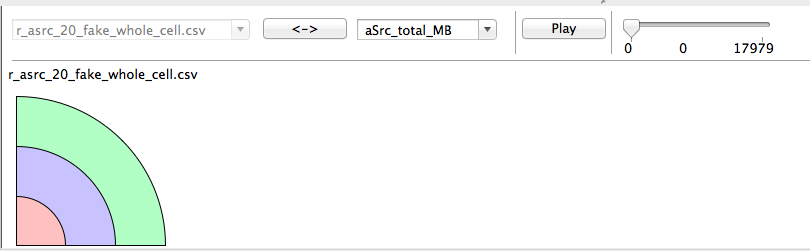
\includegraphics[width=\textwidth]{images/species_focussed.png}
        \caption{Animations Drawn in Species Focussed Manner}
        \label{fig:species_focussed}
    \end{subfigure}

    \begin{subfigure}[b]{0.9\textwidth}
        \centering
        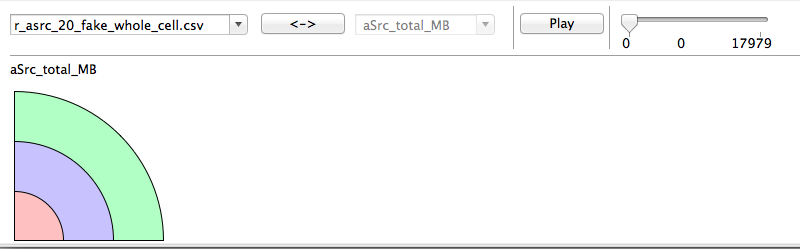
\includegraphics[width=\textwidth]{images/file_focussed.png}
        \caption{Animations Drawn in File Focussed Manner}
        \label{fig:file_focussed}
    \end{subfigure}
    \caption{The Two Ways of Drawing Animations:  File Focussed and Species Focussed.}
    \label{fig:species_file_focussed}
\end{figure}

It had been hoped to allow the user to save the animation.  This could have either been allowing the user to save individual frames or allowing them to save an animated gif of the whole animation.  Saving to a gif was chosen as it was felt to be more useful to a user to be able to export the entire animation rather than a single frame of it.  Allowing the user to save a single frame would be added in at a future date.  To generate the gif we need to save all frames.  As these frames are generated as needed, not prerendered it was required to run through the whole animation to save each frame.  This meant that saving all the frames took as long as the animation took to run.  At this step hundreds of static images have all been saved.  Then a shell script is required to convert the saved frames into a gif.  Given that this was a very slow and user unfriendly approach the decision was made to remove the ability to save animation from the project.  It would be implemented if future work was to be performed.

\section{Annotation}

Annotation was an important feature to add.  It is one of Grinstein's features that data visualisation software should have~\cite{gg_vizbi}.  This is because the purpose of a visualisation is to aid analysis.  If you have a print out of a visualisation you are able draw on it and highlight areas of interest.  Users need to be able to do this on digital versions of their visualisations.  As well as helping users analyse their data, being able to annotate also means that images for presentations can be prepared without having to save the visualisation and open it in an external program.  If you did this and then wanted to change the visualisation you would have to re-annotate it.  This is frustrating for a user and wastes their time.  Being able to do it from within the visualisation solves this problem as the raw data and the annotation data are together.  Another benefit of being able to annotate is having another way of attaching additional information to the visualisation when sending it to a colleague. Having this information on the visualisation saves them from flicking back and forth from an email or other supporting documentation.

Implementing annotation of the visualisations on offer in this tool had to be done in two parts.  This is because there are two parts to the annotation.  The graph and the cell level view.  One is a static visualisation and one is a dynamic visualisation.  Each of these required a different approach.  These are detailed below.

\subsection{Annotation of the Graph}

Annotation on the graph was relatively straightforward to implement.  matplotlib provides annotation capabilities in two forms.  One form is annotations that use arrows with or without text, and the other is arbitrary drawing on the graph.  Both of these forms have been utilised for annotations.

Users of the new tool are provided with four annotation types: arrow, text, arrow with text and circles.  Buttons for each of these annotation types have been placed on the matplotlib toolbar.  This can be seen in Figure~\ref{fig:annotation_demo}

\begin{figure}[h!]
    \centering
    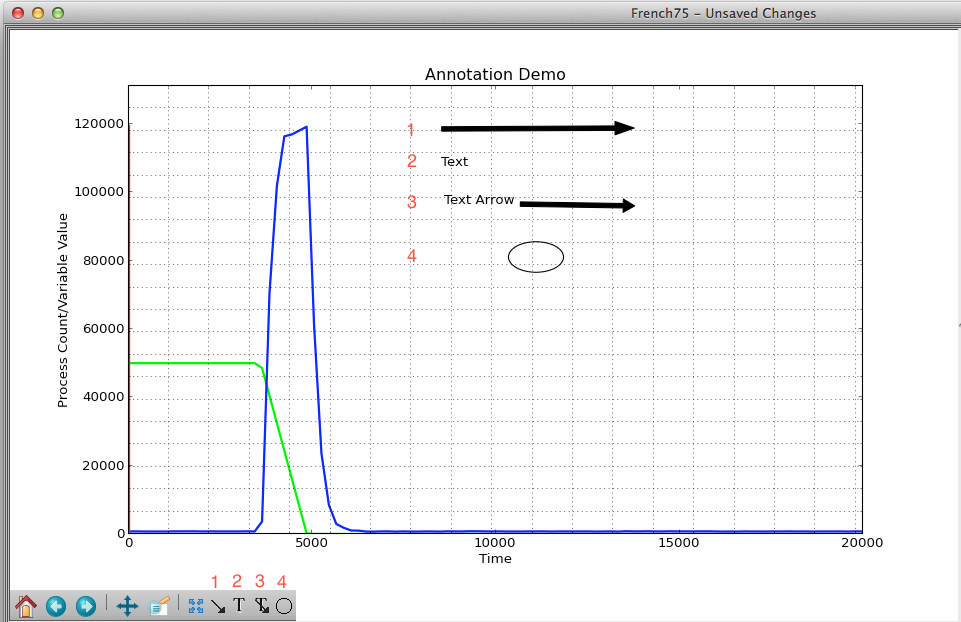
\includegraphics[width=\textwidth]{images/annotation_demo.png}
    \caption{Example of Each of the Four Annotation Types and the Toolbar Buttons that Correspond to Them}
    \label{fig:annotation_demo}
\end{figure}

There were problems in making the annotation creation process user friendly.  For all of the annotations the user needs to first press the appropriate button on the on the toolbar.  The next actions depend on the annotation type.  Text and circle annotations were intuitive as all they require is one click.  The user clicks where they want the annotation to be placed and it will be drawn on the graph there.  However the two arrow annotation types required two clicks.  The first click marks the start point (the tail of the arrow) and the second click is the finish point (the head of the arrow).  This was not obvious, when handed over to the users they didn't know that it required two clicks and didn't know whether the arrows would be drawn head to tail or tail to head.  The technique for placing arrows was changed so that the first click still fixed the position of the tail of the arrow. However the behaviour after the first click has changed, now a temporary annotation is continuously redrawn that has the head of the arrow wherever the mouse is.  This allows the user to see the arrow they are drawing.  To indicate to the user that they need to click on the graph the cursor is changed after pressing one of the annotation buttons on the toolbar.  The use of different cursors is a common technique to help guide users to perform actions.

It was important that annotations could be edited or deleted.  The annotations can not just be clicked as they are not a \ac{UI} widget like a button.  The solution to this was to have an array of annotations.  When a user right clicks on the graph it searches through all annotations and selects the annotation that was closest to the click (if that distance was below a certain threshold).  The selected annotation is then highlighted red, and a context menu appears to give feedback to the user that they have successfully selected an annotation.  This can be seen in Figure~\ref{fig:annotation_selection}  The context menu then gives the user the option to edit or delete an annotation.  Editing an annotation only allows for editing text.  For changing position the annotation has to be deleted and redrawn.

\begin{figure}[h!]
    \centering
    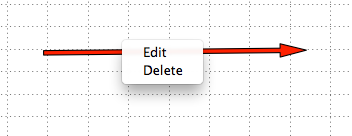
\includegraphics[width=\textwidth]{images/annotation_selection.png}
    \caption{Context Menu on Selection of Annotation}
    \label{fig:annotation_selection}
\end{figure}

To calculate the distance from the location of the mouse click to the annotation two problems had to be solved.  The first was how to calculate the distance from a point to a line.  An equation for this can be seen in Figure~\ref{fig:point_to_line_eq}.  Equation~\ref{eq:line} is the equation for a line in two dimensions.  This represents the annotation.  The equation can be calculated from the start and end points of the annotation. Equation~\ref{eq:point} is the position of the mouse click.  Equation~\ref{eq:distance} shows the equation for calculating the distance from the point to the line.  The second problem that had to be overcome was the difference in scale.  In effect we have two coordinate systems.  The results coordinate system and the visual coordinate system.  These difference are illustrated in Figure~\ref{fig:distance_scale}.  The annotations in Figure~\ref{fig:distance_scale_a} are further away from each other in the results coordinate system than the annotations in Figure~\ref{fig:distance_scale_b}, however they are closer in the visual coordinate system.  When selecting an annotation the user is using the visual coordinate system but the distance is calculated using the result coordinate space.  This could lead to the wrong annotation being selected.  The solution to this was to transfer one coordinate system into the other.  When calculating the distance from the point to the line the values are scaled by the size of the graph.

\begin{figure}[h!]
    \centering

    \begin{subfigure}[b]{\textwidth}
        \centering
        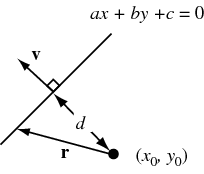
\includegraphics[width=0.3\textwidth]{images/point_to_line.png}
        \caption{Diagram of the Point to Line Distance Problem}
        \label{fig:point_to_line_diagram}
    \end{subfigure}

    \begin{subfigure}[b]{\textwidth}
        \begin{subequations}
            \begin{align}
            & y = -\frac{a}{b}x - \frac{c}{b} \label{eq:line}\\
            & (x_{0}, y_{0}) \label{eq:point} \\
            & d = \frac{\mid ax_{0} + by_{0} + c \mid}{\sqrt{a^{2} + b^{2}}} \label{eq:distance}
            \end{align}
        \end{subequations}
        \caption{Equations for Calculating the Distance From a Point to a Line.}
        \label{fig:point_to_line_equations}
    \end{subfigure}
    \caption{Equations and Diagram for Calculating the Distance From a Point to a Line (taken from WolframMathWorld~\cite{point_to_line})}
    \label{fig:point_to_line_eq}
\end{figure}

\begin{figure}[h!]
    \centering
    \begin{subfigure}[b]{0.6\textwidth}
        \centering
        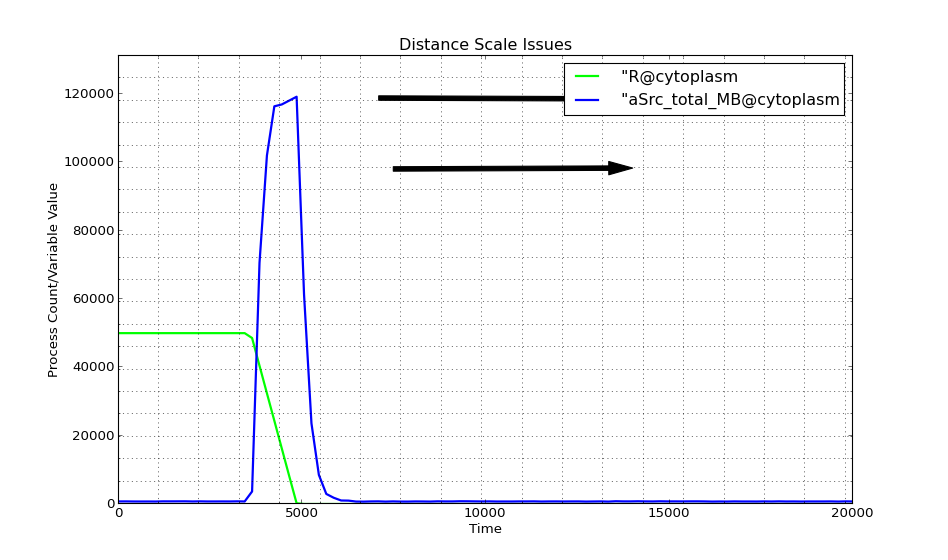
\includegraphics[width=\textwidth]{images/distance_scale_a.png}
        \caption{Annotations With Distance of Approximately 20000}
        \label{fig:distance_scale_a}
    \end{subfigure}

    \begin{subfigure}[b]{0.6\textwidth}
        \centering
        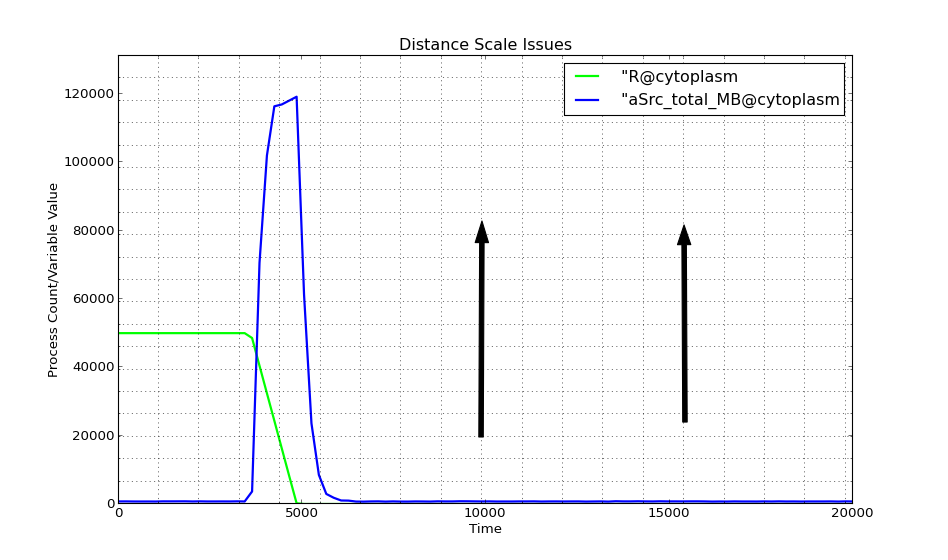
\includegraphics[width=\textwidth]{images/distance_scale_b.png}
        \caption{Annotations With Distance of Approximately 5000}
        \label{fig:distance_scale_b}
    \end{subfigure}
    \caption{Two Sets of Annotations Illustrating the Problems When Calculating Distance to an Annotation}
    \label{fig:distance_scale}
\end{figure}

A similar issue to the difference in scale when calculating the distance from the mouse to annotation was encountered when switching the graph to normalised mode.  When normalised the graph in the y axis only goes between 0 and 1.  The coordinates of the annotation are likely to be very much outside this range and the annotation would not appear on the graph.  The solution was to if the graph is normalised then to also normalise the positions of the annotations when drawing them.  A side effect of this technique is that the lines are potentially going to rescale themselves.  This could leave an annotation point to nothing.  This is unavoidable as the annotation has no concept of what it is pointing at.  It may be pointing to the intersection of more than one line, in this case it would be impossible to keep the annotation pointing at what it was originally pointing at.  Neither of these is optimal.  Both approaches lose the information that the user originally added.  During user evaluations, when the annotation would not be visible during data normalisation, the user was very confused as to why their annotation had disappeared.  It was therefore decided to have the annotation be visible but most likely incorrect as it is clearer to the user what has happened.

\begin{figure}[h!]
    \centering
    \begin{subfigure}[b]{0.6\textwidth}
        \centering
        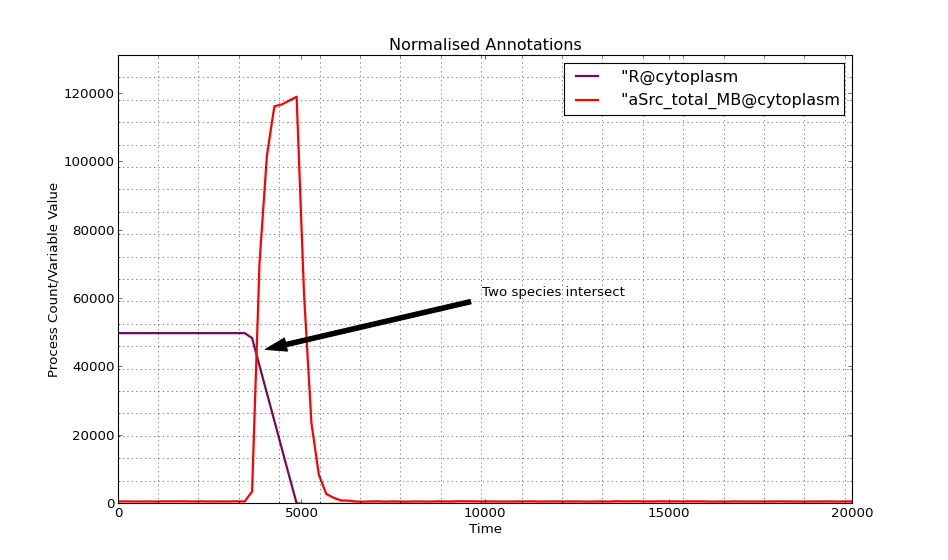
\includegraphics[width=\textwidth]{images/unnormalised_annotation.png}
        \caption{Annotation Pointing at Correct Intersection of Species}
        \label{fig:distance_scale_a}
    \end{subfigure}

    \begin{subfigure}[b]{0.6\textwidth}
        \centering
        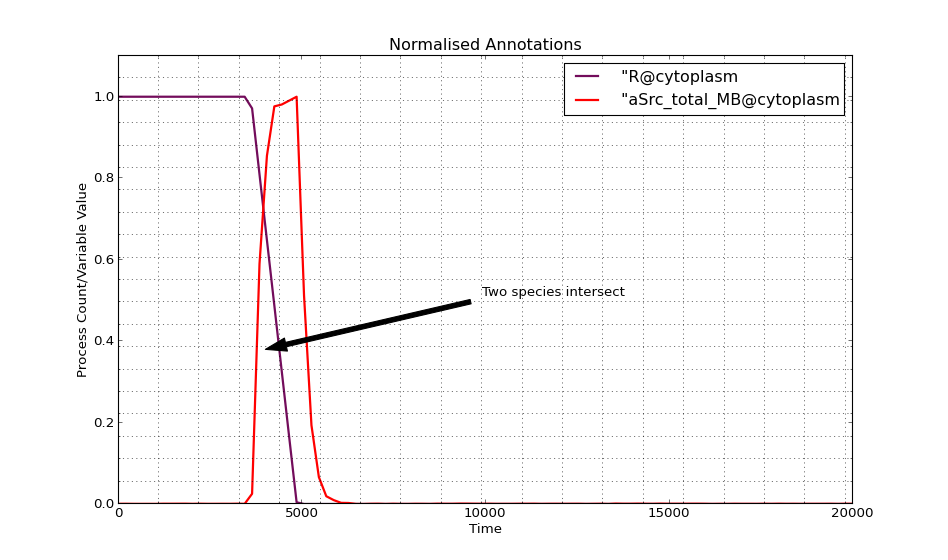
\includegraphics[width=\textwidth]{images/normalised_annotation.png}
        \caption{Annotation Pointing at Nothing After Data Normalisation}
        \label{fig:distance_scale_b}
    \end{subfigure}
    \caption{Graphs Illustrating What Happens to Annotations Whilst Data is Normalised}
    \label{fig:distance_scale}
\end{figure}

\subsection{Annotation of the Animation}
\label{sec:anime_annotation}

After completing annotation of the graph it was important to expand this to the animation panel, as this is the other visualisation option available to a user.  Annotating animations posed more of a challenge than annotation of the graph and there were a number of issues to overcome.

\begin{enumerate}
\item How to implement the annotations?  For the graph matplotlib has built in annotation support.  wxPython does have drawing support but not in built annotation support.  Annotating on the animation will need manual handling of the drawing on top of the animation visualisation.  Manual drawing means that the automatic layout functionality that wxPython provides cannot be used.
\item When to display the annotations?  When an annotation is drawn on the graph it is displayed at all times.  The appearance of the graph does not change over time.  However the appearance of the animation visualisation does change over time.  The problem faced when annotating is whether to have annotations available at only specific times in the animation, or to have them there the whole time, and if they are going to appear and disappear how can it be done without being distracting?
\item How to give the user control over the annotations? When a user wants to edit or delete an annotation on the graph it is always there.  However on the animation panel if the annotation is temporal, then it is not always visible for the user to edit or delete and it would be frustrating for a user to constantly have to search through the animation to look for annotations to change them.
\end{enumerate}

A platform where users are able to annotate an `animation' is YouTube~\cite{youtube}.  YouTube's annotation interface can be seen in Figure~\ref{fig:youtube}.  Youtube's approach is to allow the user to set what period of time an annotation is visible for.  There is also a management panel where the user can see all of the annotations and edit or delete them.  This approach solved issues two and three and was adapted for this tool.

\begin{figure}[h!]
    \centering
    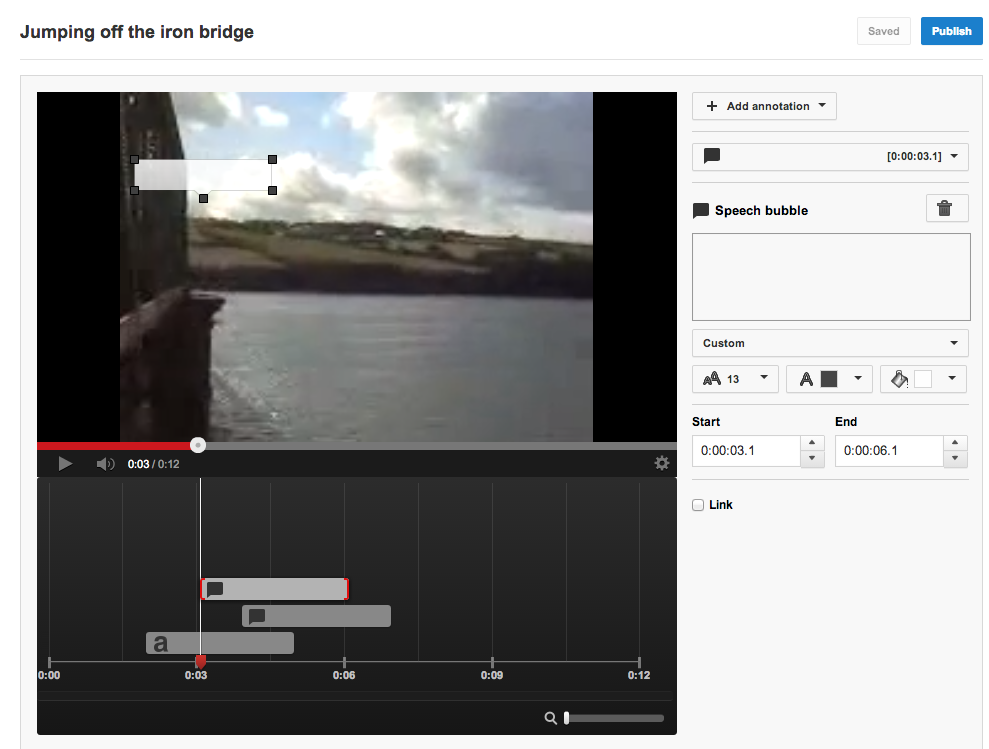
\includegraphics[width=0.7\textwidth]{images/youtube.png}
    \caption{YouTube Video Annotation Interface}
    \label{fig:youtube}
\end{figure}

On the right hand side of the tool there is a panel which lists all annotations that have currently been added to the tool, this can be seen in Figure~\ref{fig:annotatlion_list}.  This provides the user with the persistent view of what has been added.  When the user creates an annotation they are shown a dialogue that allows them to enter the annotation text and to choose a duration.  This indicates to the user that the annotation will only be visible at certain times.  The start and end times are given in model time.  The duration displayed to the user is given as the real time that the annotation will be visible for.  This can be seen in Figure~\ref{fig:annotation_dialog}.

\begin{figure}[h!]
    \centering
    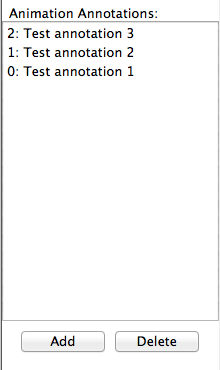
\includegraphics[height=0.4\textheight]{images/annotation_list.png}
    \caption{Animation Annotation List}
    \label{fig:annotation_list}
\end{figure}

\begin{figure}[h!]
    \centering
    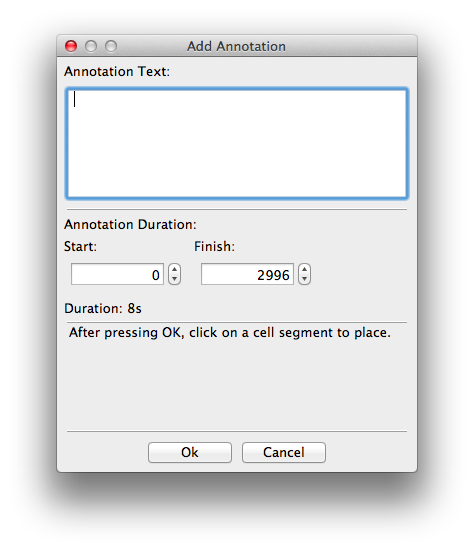
\includegraphics[width=0.7\textwidth]{images/annotation_dialog.png}
    \caption{Animation Annotation Dialogue}
    \label{fig:annotation_dialog}
\end{figure}

The first problem -- how to display the annotations -- has also been solved.  Drawing in wxPython takes place on panels.  Each cell cross section is placed on its own panel.  This drastically limits the available space.  The panels are not wide enough to have the annotation text drawn on.  The solution was to assign each annotation a number and that number is what is used to annotate the cell.  The number is then displayed in the annotation list box allowing the user to read the appropriate annotation.  This can be seen in Figure~\ref{fig:annotation_whole}

\begin{figure}[h!]
    \centering
    \begin{subfigure}[b]{0.4\textwidth}
        \centering
        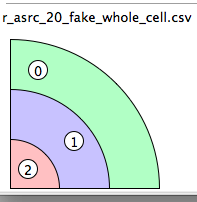
\includegraphics[width=0.9\textwidth]{images/annotation_whole_b.png}
        \caption{Annotated Cell Section}
        \label{fig:annotation_whole_cell}
    \end{subfigure}
    \begin{subfigure}[b]{0.4\textwidth}
        \centering
        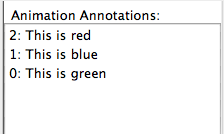
\includegraphics[width=0.9\textwidth]{images/annotation_whole_a.png}
        \caption{Corresponding Annotation List}
        \label{fig:annotation_whole_list}
    \end{subfigure}
    \caption{Animation Annotations}
    \label{fig:annotation_whole}
\end{figure}

\section{Data Mining}

Gone - WHY?

\section{Search}

Begin able to use a time series data as a query against a database of time series data was one of the new goals added to the project.  It was felt it would be of great use to the biologists as it would allow for discoverability within the tool. \tdi{Find a citation that backs this as being useful}.  It is also a feature in the tool that incorporates cross domain knowledge in an area of active research.

Some problems needed to be overcome before using plots as a query was useful:
\begin{itemize}
\item How to cope with different scales?
\item How to cope with events happening at different times?
\item How to represent the plot to allow for efficient search?
\item How to determine similarity between two graphs?
\end{itemize}

Early techniques used simple similarity measures such as Euclidean distance, but these gave poor results.  The reason for the poor results is that Euclidean distance does not take into account scale or time.  Figure~\ref{fig:similar} illustrates a case where Euclidean distance would give a poor similarity measure.  The two lines are identical, but the green line has been shifted in time.  Euclidean distance will not recognise that they are similar.  The same problem would happen if one line had been shifted in the y-axis above the other.

\begin{figure}[h!]
    \centering
    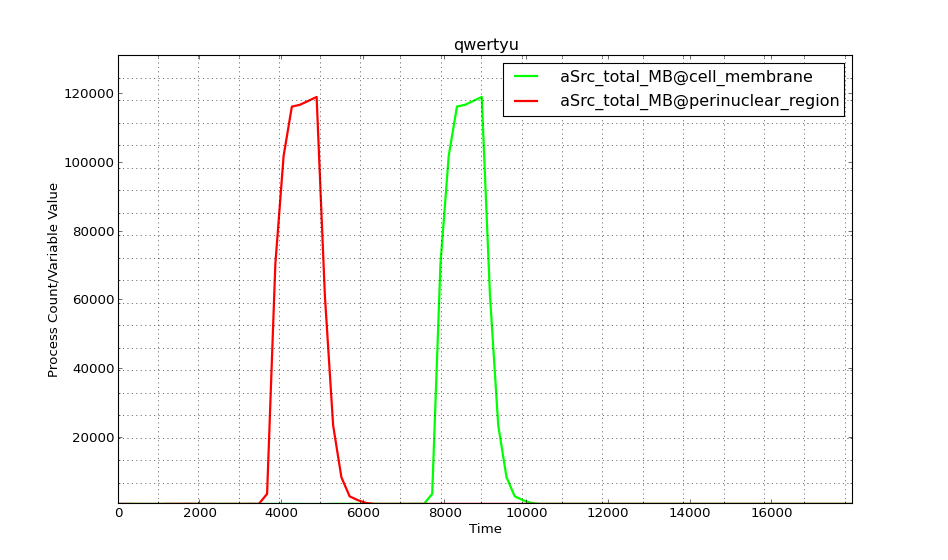
\includegraphics[width=0.7\textwidth]{images/similar_plots.png}
    \caption{Identical Plots Shifted in Time}
    \label{fig:similar}
\end{figure}

It is important to define what it means for two lines to be similar.  It is obvious that in case such as Figure~\ref{fig:similar} that the two lines are similar.  Both lines are the same shape, they are exhibiting the same behaviour.  When determining similarity of plots we should take a time invariant approach.  Perhaps less obvious is the case where we have offset in the Y-Axis as shown in Figure~\ref{fig:similar_y}.  Figure~\ref{fig:similar_1} shows two identical lines where one line had an initial 100000 population level.  Figure~\ref{similar_2} shows two lines where one line is double the other line.  Figure~\ref{fig:similar_1} is effectively the same case as Figure~\ref{fig:similar}.  Figure~\ref{fig:similar_2} is different, but it is clear looking at the graph that they are exhibiting the same behaviour.  when determining the similarity of plots we should take a scale invariant approach. \tdi{dig out some citations for this}

\begin{figure}[h!]
    \centering
    \begin{subfigure}[b]{0.6\textwidth}
        \centering
        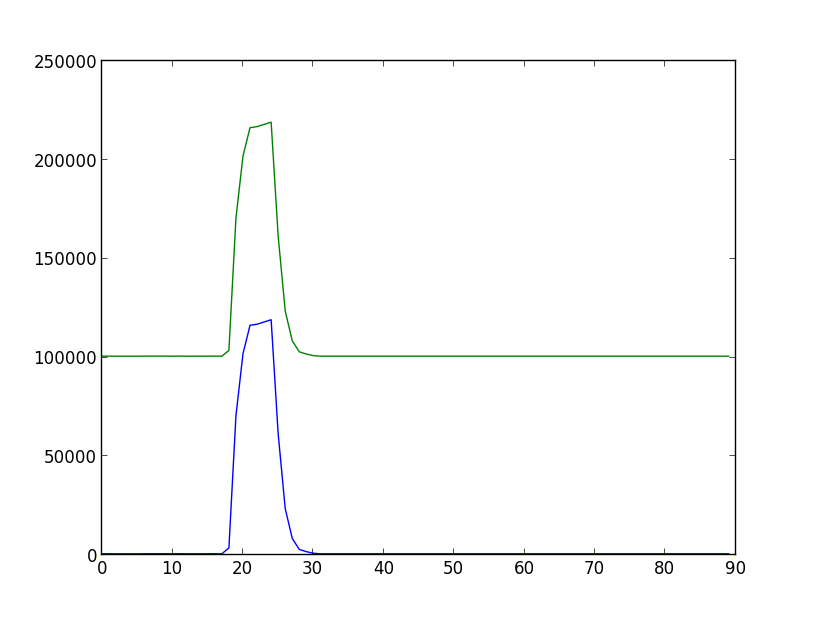
\includegraphics[width=0.7\textwidth]{images/similar_plots_2.png}
        \caption{Identical Plots Shifted in Population Level}
        \label{fig:similar_1}
    \end{subfigure}

    \begin{subfigure}[b]{0.6\textwidth}
        \centering
        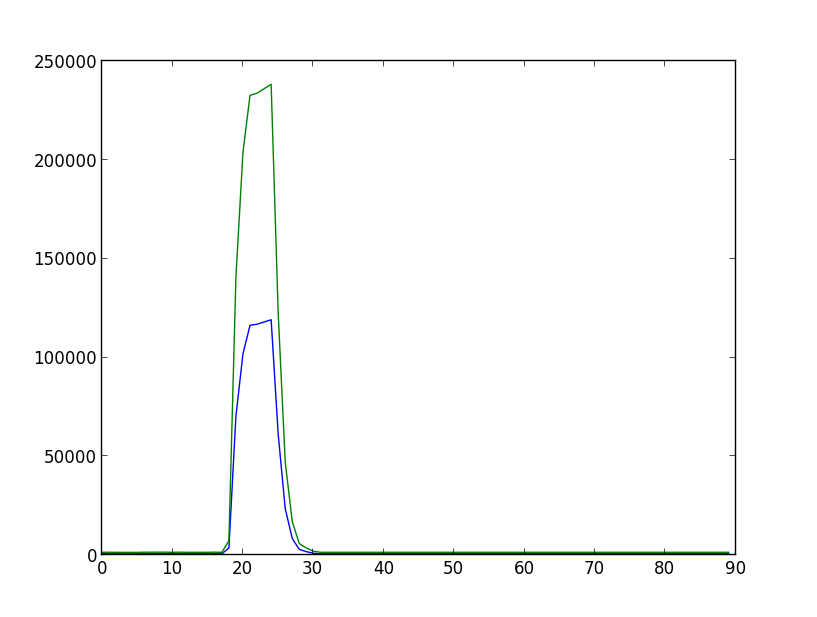
\includegraphics[width=0.7\textwidth]{images/similar_plots_3.png}
        \caption{Identical Plots Scaled in Population Level}
        \label{fig:similar_2}
    \end{subfigure}
    \caption{Graphs Illustrating Different Ways Lines can be Offset in the Y-Axis}
    \label{fig:similar_y}
\end{figure}

Approaches that have been researched to determine similarity between time series data have included shape based approaches and dynamic programming techniques.  Not all of these approaches lent themselves to fingerprinting.  A necessary feature for efficient querying.  After researching alternatives an approach was adapted from the work of Lin \& Li~\cite{structural_similarity}.

Their approach uses normalised sub sequence data to reduce the dimensionality of the dataset and build a fingerprint.  This fingerprint can then be used to efficiently find the most similar plots in the database.  This approach is explained in further detail below:

The first step is to take the input data and using a sliding window to create the sub lists.  The size of the sliding window will determine the word size in the fingerprint.  Lin uses a size of 8 for the sliding window.  The same value was chosen here.  If we have input data $[1,2,3,4,5]$ and windows size $n = 3$ then we get the sub lists as $[[1,2,3]$, $[2,3,4]$, $[3,4,5]]$

The second step is to normalise each sub list.  Each sub list is normalised to be zero mean and unit variance.  This places each sub list onto the same scale.  This removes the effect of the offsets seen in Figure~\ref{fig:similar_y}.  To normalise to zero mean and unit we need the mean ($\mu$) and the standard deviation ($\sigma$).  We then have:

$$
\left[\frac{X - \mu}{\sigma},\text{   } x \in sublist\right]
$$

The third step is to reduce the dimensionality of the data and build the fingerprint.  Lin's approach also involves converting the data from a continuous representation into a discrete representation.  By normalizing the sub lists to be zero mean and unit variance we allow a Gaussian distribution to be fitted to the data.  This can be seen in Figure~\ref{fig:gaussian_plot}.  This approach does assume the Gaussian distribution is a suitable distribution.  Lin found it to be a suitable distribution but does note that other distributions could be investigated, this was outside the scope of this project.  For each data point we use the Gaussian function and map it to a letter.  This can be seen in Figure~\ref{fig:gaussian_plot}.  Lin uses three characters and found it to be suitable, again alternative numbers of characters could be used but this is outside the scope of the project.  This builds up a fingerprint of the graph with much reduced dimensionality.

\begin{figure}[h!]
    \centering
    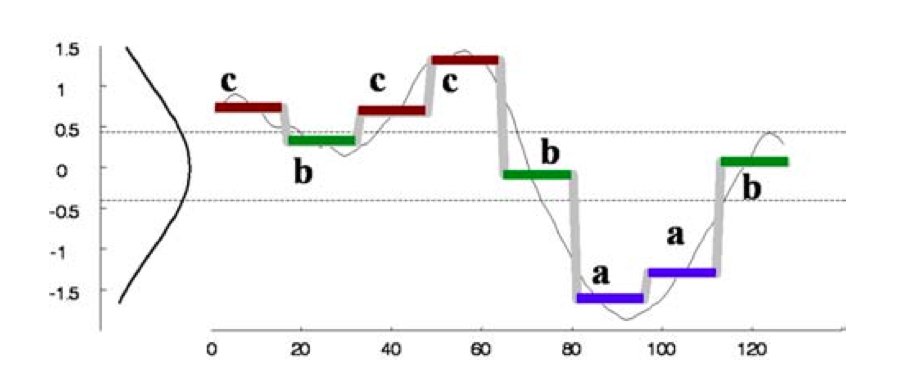
\includegraphics[width=\textwidth]{images/similiarty_normalise.png}
    \caption{Fitting Gaussian to Time Series Data, taken from~\cite{structural_similarity}.}
    \label{fig:gaussian_plot}
\end{figure}

Our fingerprint of the plot is now a list of words.  Lin now calls for the removal of local duplicates of words.  If we have runs of a certain word then that should be reduced to a single instance of the word.  For example if we have the fingerprint $"AAA", "AAA", "BBA", "BBB", "BBB", "AAA", "AAA"$ it should be reduced to $"AAA"$, $"BBA"$, $"BBB"$, $"AAA"$ not $"AAA"$, $"BBA"$, $"BBB"$.  We are not removing all duplicates of the word.  This reduces the number of entries in the fingerprint and provides an efficiency benefit.  It will also remove the effect seen in Figure~\ref{fig:similar_2} where Euclidean distance would fail if one line is a scaled version of the other.

We now have a fingerprint of the plot.  The fingerprint is a list of strings.  Our strings all have a length of eight characters, the strings are composed from a three letter alphabet.  This gives us a vocabulary of $3^8$ possible words.  The fingerprint is a $3^8$ element vector where each entry in the vector contains the count of the word in the line.  This is a very wasteful representation as most of the entries in the vector will be zero.  We can replace this with a sparse representation of the fingerprint where we store what words make up the line and their count.

This fingerprint representation of the plot also solves the problem of features being temporally located in the graph.  In the fingerprint there is no ordering of the words, in effect all the features happened at the same time.  This is a common representation in information retrieval and is referred to as bag-of-words.  A more suitable name in this domain would be bag-of-features.

Now that we have a representation of the plot that is scale and time invariant and allows for efficient comparisons we can find a method to calculate the similarity.

We could simply just use Euclidean distance again, using the two fingerprints as the input, but this does not do anything to weight rarer features.  If two plots have rare features in common then that is much more significant for similarity than if they share very common features.  A similarity measure that takes into account the importance of a word is therefore desirable.

It was decided to implement tf.idf weighted cosine as the similarity measure.  This takes into account term frequencies to provide a higher weight to rarer vectors.  tf.idf is very well researched in the field of information retrieval and text mining.  Given the representation of the finger print is equivalent to a bag-of-words it seems sensible to apply tf.idf to this domain.  A description of how tf.idf weighted cosine works can be found in Section~\ref{sec:tfidf}.

The tf.idf weighted cosine similarity~\cite[p.~243]{se_book} can then be calculated between the query plot and each individual plot in the database.  These similarity scores can then be ranked.

\subsection{tf.idf}
\label{sec:tfidf}

\ac{tf.idf} is a technique for calculating how important a word is to a document.  \ac{tf.idf} requires a corpus of document vectors.  With the corpus data \ac{tf.idf} can take as input a query vector and transform that into a vector of weights, where the weights are the \ac{tf.idf} scores of each word.

\tdi{Why do we care about weighting words}

Equation~\ref{eq:tfidf} is the equation for finding the similarity between a short query term and a longer document.  This equation would be applied between the query term and every document in the corpus.  This would then give a similarity ranking.  Below is an explanation of the components of the equation and how they affect the weighting of a word.

\begin{itemize}
    \item $tf_{w,Q}$ -- The number of times word $w$ appears in query $Q$.  If a word is repeated in the query it is likely to be important.
    \item $tf_{w,D}$ -- The number of times word $w$ appears in document $D$.  If a word is repeated in the document it is likey to be important.
    \item $k$ -- A squashing factor.  The first occurrence of a word is more important than repeats.
    \item $|D|$ -- Length of the document
    \item $|C|$ -- Number of documents in the corpus
    \item $df_{w}$ -- Number of documents in the corpus that contain word $w$
    \item $avg|D|$ -- Average length of all documents in the corpus.
    \item $tf_{w,D} + \frac{k|D|}{avg|D|}$ -- Normalising factor, repeated words are less important unless the document is longer than average.
    \item $\log \frac{|C|}{df_{w}}$ -- Increases the weighting of words that are rare across the corpus.
\end{itemize}

Equation~\ref{eq:dw} is the equation for calculating the \ac{tfidf} weighting of a single word in document vector.  This equation would be applied to every word in the document vector and transform the document vector into the document's weight vector.

Equation~\ref{eq:tfidf_cosine} is the equation for \ac{tfidf} weighted cosine similarity.  This gives a better measure of similarity when comparing the query is a document as is the case here \tdi{Citation for this is tts lecture slides is this ok?}.

\begin{subequations}
    \begin{align}
    s(Q, D) &= \sum_{w} tf_{w,Q} \times \frac{tf_{w,D}}{tf_{w,D} + \frac{k|D|}{avg|D|}} \times \log{\frac{|C|}{df_{w}}} \label{eq:tfidf}\\
    D_{w} &= \frac{tf_{w,D}}{tf_{w,D} + \frac{k|D|}{avg|D|}} \times \log{\frac{|C|}{df_{w}}} \label{eq:dw}\\
    S(D_{1}, D_{2}) &= \frac{\sum_{w} D_{1,w} \times D_{2,w}}{\sqrt{\sum_{w} D_{1,w}^2} \times \sum_{w} D_{2,w}^2} \label{eq:tfidf_cosine}
    \end{align}
\end{subequations}

\tdi{Talk about indexing}

\ac{tf.idf} allows for efficient search through the use an index and an inverted index.  The index is a mapping from document to words and the inverted index is a mapping from words to documents.  If we look up a document we find what words are in it.  If we look up a word we find what documents contain it.  When a new plot is added to the database these two indexes are updated.  With these two indexes all the components of \ac{tfidf} can be calculated for very little cost.  For example $tf_{w,D}$ would involve looking up document D in the index, this will return to us all the words in document D and their counts.  We can then quickly find the count of word $w$ in $D$.

\subsection{Results}
\tdi{move this into evaluation?}
Initial results are very promising with the tf.idf weighted cosine providing much clearer results than with simple euclidean distance.  There is not a large enough truth set of plot similarities to be able to confidently say that it is effective.  However these early promising results seem to indicate that further research would certainly be worthwhile, but outside the scope of the project.

DISCUSSION OF THE EARLY RESULTS

\section{Real Time Collaboration}

More and more programs are allowing their users to collaborate in real time.  Some of these pieces of software are discussed in Section~\ref{sec:review}.  Only one piece of software could be found that was biology focused.  Implementing real time collaboration in this tool is therefore a great advantage.

There are two broad ways that real time collaboration could have been implemented: in a distributed manner or by having a single centralised instance.  A single centralised instance is the approach taken by all the software reviewed.  The approach taken in this tool is the distributed approach.

The single centralised approach would have been simpler.  With the distributed approach you have to ensure that each instance of the program has the same ordering of events and is displaying the same state.  In the centralised approach there is a single repository which has all history of what has happened.  The order that the single program instance thinks events happens in is the order that those events happened in.

Ideally the collaborative model used would have been the centralised model.  This would however have required a significant reworking of how the tool worked.  All the software reviewed was browser based.  Given the time constraints on the project and the fact that it had been developed up until this point as a standard desktop application it was felt it would be easier to implement distributed collaboration.

The collaboration that has been implemented in this project is only between two program instances.

The first stage in allowing distributed collaboration was enabling the different program instances to talk to each other. There are a number of techniques to allow for this.  Data could have been sent directly through sockets, another option would be to create a web server and send get requests and pass parameters.  It was decided to use an existing library to handle the communication.  The library chose was simplexmlrpc.  This allows each instance to run a client and a server.  The server has an api and this can be called.

On initial connection the `master' sends its entire session state the the `slave' uses this as its initial state.  After this whenever either client performs an action it issues a call to the other clients server to perform the same action.

This approach was not without its problems.  A fundamental problem with having the collaboration follow a distributed model is how to ensure that both program instances have the same ordering of events.  To solve this problem Lamport clocks were used.  Any action that affects the session state, an action that does this is one that will need to be sent to the collaborators, increments the Lamport clock.  The Lamport clocks are then sent with every message.  When a message arrives the program checks the Lamport clock and works out where in the history it should go.  After reordering the history all the visualisations are redrawn.  This also has to be done in the instance of the program that is sending the change.

Another issue that was encountered was to do with how the program was architected.  The session data was often directly modified by methods that were bound to \ac{UI} elements.  These methods are also the ones that called the client to send the message to the collaborator, if the server on the other end then called the same method to perform the action it would have resulted in an infinite loop.  These methods would also often do more than just modify the state, for example when modifying an annotation the method will find the appropriate annotation and edit it.  The client would then send a message saying delete annotation 1.  The server would not be able to call the original method as it doesn't take a parameter.  The solution to this was to split the methods up more.  Now the more typical flow is the \ac{UI} bound method calls another method that modifies the state.  The server is able to call the same method.  This removes the need for duplicated code.

\begin{figure}[h!]
    \centering
    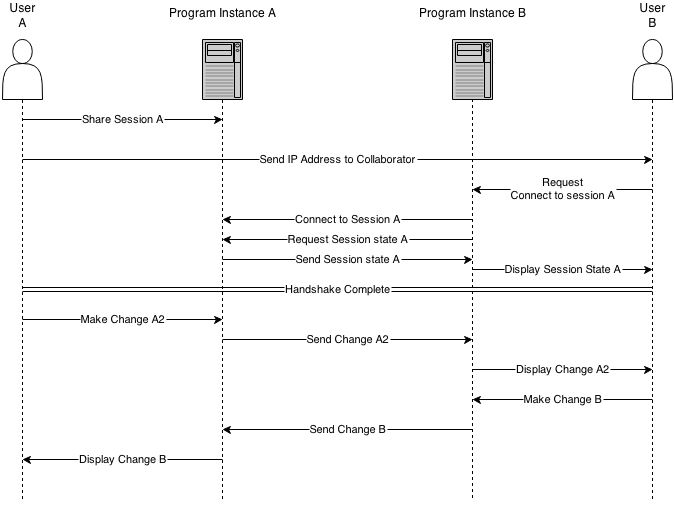
\includegraphics[width=\textwidth]{images/minf_collab_diagram.png}
    \caption{Collaboration handshake stage}
    \label{fig:collab_handshake}
\end{figure}

\begin{figure}[h!]
    \centering
    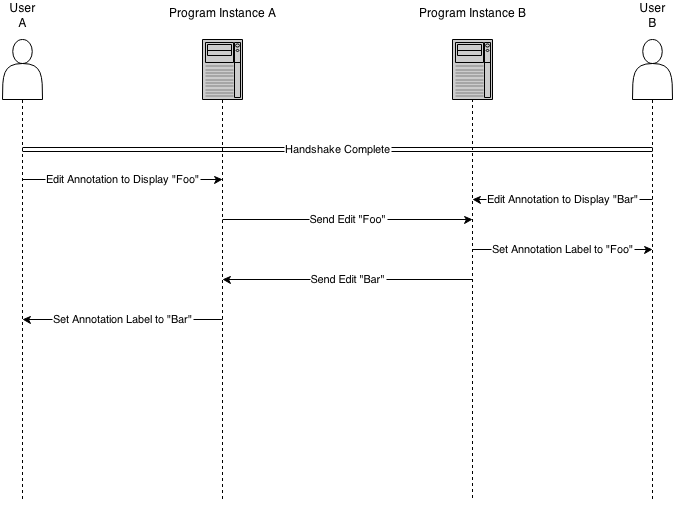
\includegraphics[width=\textwidth]{images/minf_collab_mixup.png}
    \caption{Out of sync collaboration}
    \label{fig:collab_mixup}
\end{figure}

\begin{figure}[h!]
    \centering
    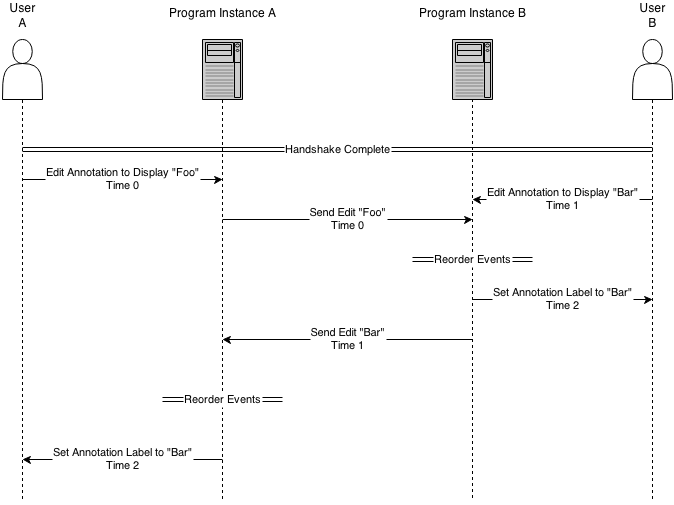
\includegraphics[width=\textwidth]{images/minf_collab_mixup_fix.png}
    \caption{Use of Lamport clocks to keep collaboration in sync}
    \label{fig:collab_mixup_fix}
\end{figure}

\begin{figure}[h!]
    \centering
    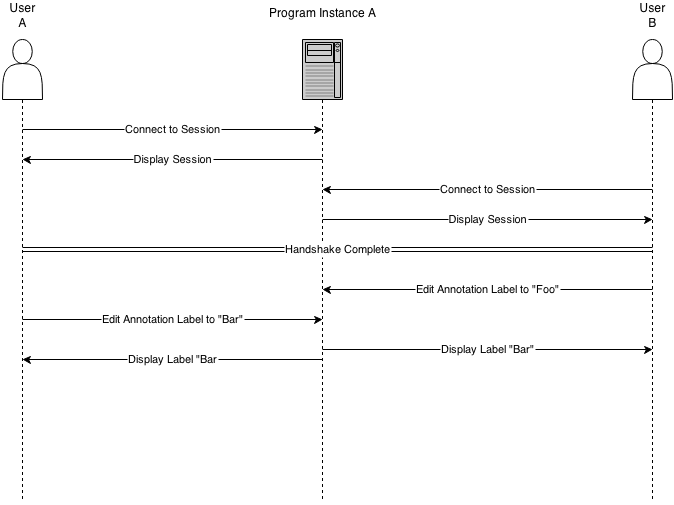
\includegraphics[width=\textwidth]{images/collaboration_single_instance.png}
    \caption{Communication flow in a centralised mode}
    \label{fig:collab_mixup_fix}
\end{figure}


\section{Usability}

In all the evaluations of the project users have commented on the difficulty of using parts of the tool.  Action has been taken to make it easier to use.  Many of the changes have been guided by Shneiderman, Norman \& Nielson's guidelines.  Specifics are detailed below.

\subsection{Undo \& Redo}
Shneiderman calls for easy reversal of actions and Nielson calls for user control and freedom -- an emergency exit from an unwanted state.  To address this, an undo/redo functionality has been added.  This required refactoring of the project code, so that the session data is in one location, inside a singleton. Any changes to this data are picked up during the next \ac{UI} update and are reflected in the visualisations.  The session data is stored as a dictionary.  To implement undo and redo, copies of the data dictionary are pushed and popped onto the stack.  Copies are pushed onto the undo stack on any atomic change the user makes.  This gives the user a full session history to go back through and this was one of the early goals from the first project phase.

A problem was encountered when trying to copy the dictionary onto the stack.  When just pushing the dictionary onto the stack it would not put a new copy of it onto the stack, so any changes to the dictionary after it has pushed onto the stack are also there in the stack.  Python dictionaries have a copy method.  Copy only does a shallow copy -- any objects in the original dictionary will have their reference placed in the new dictionary.  This was fine for some parts of the session dictionary, but for others it was not. In particular, lines and annotations, which are custom objects presented problems.  This was solved by using deep copy.  With deep copy a new copy is made of objects as well.  Some elements of wxPython and matplotlib were unable to be deep copied, but this was fixed whilst focusing more around the data -- so the \ac{UI} elements use the data, not the other way around.

\subsection{Saving}

It is important that a user is able to save and load the visualisation session as they may not be able to complete all their analysis in one sitting and may want to come back to their work in the future.  Without the ability to save and load the user would have to repeatedly add annotations and change preferences and attach files.  It was possible to add Saving and loadingby building on the work done to implement undo \& redo, although further work was required. Python has a module called pickle to serialise and deserialise data.  When saving, the dictionary containing the session data is pickled and written to a file and when loading the reverse happens.  Because the program is now focused on the data model, once a previous session has been loaded, a \ac{UI} refresh is triggered and the visualisation reflects the loaded data.

Saving the data also enables limited collaboration.  The user can customize the appearance and add annotations.  They can then save the state to a file and email that file to a colleague.  The colleague can then load the file and see the user's work.  The colleague can then correct any issues and add their own work.  The colleague can then save this and email it back to the user.  This is useful and is better than no collaboration, but it is entirely non realtime.

\subsection{Feedback}
Norman and Shneiderman both call for feedback to be given to the user so that the user can be sure that an action has been accomplished.  This feedback can come in a number of different forms and was in place in some parts of the project already.

Existing feedback in the project was a natural byproduct of some of the features; for example, when loading a results file the feedback that the load operation has been successful is that a graph appears on the screen. If the graph does not appear then something has gone wrong.  Additional feedback has been added to the project:
\begin{itemize}
\item When adding annotations the cursor changes to indicate to the user that they can interact with the graph in a different way.
\item The title bar text changes to display ``unsaved'' when the user makes a change and then changes back to ``saved'' when a successful save has been performed.
\end{itemize}

\subsection{Guiding the User}

The first evaluation of the second phase of the project unearthed that the users struggled to choose the correct action as there were multiple ways of doing the same action that had slightly different use cases.  There was also confusing language in the menu options.  These multiple paths have been removed. For example, now there is only one way to open results files initially.  To help guide the user further \ac{UI} elements are enabled and disabled as appropriate.  Now when the program is first loaded the only action a user can perform is to load a session or start a new session.  Afterwards other \ac{UI} elements are enabled to allow the user to start using the tool effectively.

The requirement of the model file for parsing animation has also led to animation replacing the previous model visualisation.  In the set up phase after the the model and the species have been parsed the user is presented with a cell segment, similar to what is seen in the animation panel.  The cell segment is split into different regions, one for each region of the cell.  These segments are then coloured if the selected species is present in them.  The user can select between all species in the selected results files.  This has a number of benefits.  First, they can sanity check that they have matching results and model files.  Second, they can see how the model is structured.

To make setting up the animation user friendly to control required the model file so that the location hierarchy could be parsed.  Before this there was an awkward system where the user had to input where in the cell a species is.  This was time consuming, awkward and quite brittle.  At the time it assumed that there would be three compartments in the species, which is a terrible assumption to make.

\section{Data Manipulation and Export}
